\section{Quasar Benchmarks}

\label{sec:quasar-bench}

\subsection{Testnet Configuration}

\begin{itemize}
    \item \textbf{Validators}: 21 nodes, AMD EPYC 7763, 512GB RAM, NVIDIA A100
    \item \textbf{GPU Workers}: 500 nodes with various GPU configurations
    \item \textbf{Network}: 10 Gbps interconnect, 5 geographic regions
    \item \textbf{Block gas limit}: 1 billion
\end{itemize}

\subsection{Finality Latency}

\begin{table}[t]
\centering
\begin{tabular}{lcccc}
\toprule
\textbf{Validators} & \textbf{p50 (ms)} & \textbf{p95 (ms)} & \textbf{p99 (ms)} & \textbf{p99.9 (ms)} \\
\midrule
7 & 5.1 & 7.2 & 9.8 & 14.2 \\
21 & 6.3 & 9.1 & 12.4 & 18.7 \\
50 & 8.2 & 12.8 & 17.1 & 25.3 \\
100 & 11.4 & 18.6 & 24.9 & 38.2 \\
200 & 16.8 & 28.4 & 39.1 & 58.7 \\
\bottomrule
\end{tabular}
\caption{\Quasar{} finality latency distribution by validator count.}
\label{tab:finality}
\end{table}

\begin{figure}[t]
\centering
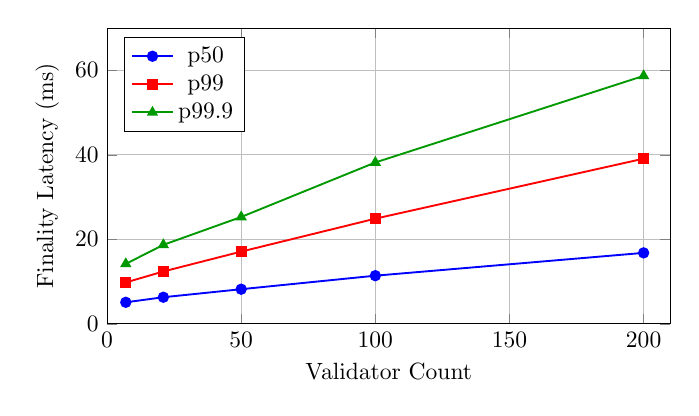
\begin{tikzpicture}[scale=0.85]
    \begin{axis}[
        xlabel={Validator Count},
        ylabel={Finality Latency (ms)},
        xmin=0, xmax=210,
        ymin=0, ymax=70,
        legend pos=north west,
        grid=major,
        width=10cm,
        height=6cm
    ]
    \addplot[blue, thick, mark=*] coordinates {
        (7, 5.1) (21, 6.3) (50, 8.2) (100, 11.4) (200, 16.8)
    };
    \addlegendentry{p50}

    \addplot[red, thick, mark=square*] coordinates {
        (7, 9.8) (21, 12.4) (50, 17.1) (100, 24.9) (200, 39.1)
    };
    \addlegendentry{p99}

    \addplot[green!60!black, thick, mark=triangle*] coordinates {
        (7, 14.2) (21, 18.7) (50, 25.3) (100, 38.2) (200, 58.7)
    };
    \addlegendentry{p99.9}
    \end{axis}
\end{tikzpicture}
\caption{\Quasar{} finality latency vs validator count. Latency scales sub-linearly due to $O(n)$ message complexity.}
\label{fig:finality}
\end{figure}

At Zoo's production validator count of 21, median finality is 6.3ms with p99 at 12.4ms.

\subsection{Throughput}

\begin{table}[t]
\centering
\begin{tabular}{lccc}
\toprule
\textbf{Validators} & \textbf{TPS (transfers)} & \textbf{TPS (mixed)} & \textbf{Blocks/sec} \\
\midrule
7 & 5,120,000 & 3,450,000 & 196 \\
21 & 4,760,000 & 3,210,000 & 159 \\
50 & 4,310,000 & 2,890,000 & 122 \\
100 & 3,780,000 & 2,510,000 & 88 \\
200 & 3,020,000 & 1,980,000 & 60 \\
\bottomrule
\end{tabular}
\caption{\Quasar{} throughput by validator count. Mixed workload: 60\% transfers, 30\% swaps, 10\% AI.}
\label{tab:throughput}
\end{table}

\subsection{Message Complexity}

\begin{table}[t]
\centering
\begin{tabular}{lccc}
\toprule
\textbf{Protocol} & \textbf{Complexity} & \textbf{Msgs (21 val)} & \textbf{Msgs (100 val)} \\
\midrule
PBFT & $O(n^2)$ & 441 & 10,000 \\
HotStuff & $O(n)$ & 63 & 300 \\
\Quasar{} & $O(n)$ & 42 & 200 \\
\Quasar{} (fast path) & $O(n)$ & 21 & 100 \\
\bottomrule
\end{tabular}
\caption{Message complexity comparison. \Quasar{} achieves fewer messages than HotStuff via pipelining.}
\label{tab:messages}
\end{table}

